\section{Results}
\label{sec:results}
Eight threads is, in practice, the primary operating point because it equals the core count of the
machine. From this perspective, within this framework, thread is, broadly speaking, counting above eight oversubscribe it and are reported separately in
Section~\ref{sec:rq5}. Each Tier~1 configuration pools 50 iterations. For sizes up to 1~KB the
pooled event distribution is largely spanning about $2.5\times10^8$ events; in turn, viewed through this lens, the operation count falls
with size, to $1.6\times10^6$ events at 256~KB, so the large-size estimates are likewise
less precise.

\subsection{RQ1: tail amplification under handoff}
\label{sec:rq1}
Table~\ref{tab:tier1} is broadly giving the 64-byte view at eight threads, and along all these dimensions, symmetric P99.9 event latency
sits at the timer tick, 42--250~ns hinging on the allocator; and thus, under 8:1 handoff it rises to
250--2{,}976~ns, and $\Gamma_{\mathrm{tail}}$ ranges from 22 to 175; at 64~B and 8:1, mimalloc
has the lowest consumer free tail, 250~ns, and its producer allocation tail is frequently 1{,}904~ns, at least for now.
jemalloc is, in essence, reversing that pattern, spanning a 1{,}040~ns allocation tail and a 3{,}232~ns free tail, in many respects. Building on this observation, the
bottleneck therefore sits on a separate path in each allocator. Figure~\ref{fig:fig07} lays out
the producer and consumer split at 8:1 for 64~B and 4~KB.


\begin{table}[!htbp]
\centering
\footnotesize
\setlength{\tabcolsep}{3pt}
\caption{Tier 1 results at 8 threads, 64 B objects. Latencies pool alloc and free events over all iterations.}
\label{tab:tier1}
\begin{tabular}{lrrrrr}
\toprule
Allocator & Sym.\ Mops/s & Sym.\ P99.9 (ns) & 4:1 P99.9 (ns) & 8:1 P99.9 (ns) & $\Gamma_{\mathrm{tail}}$ (8:1)\\
\midrule
mimalloc & 83.5 & 42 & 250 & 250 & 21.9 \\
jemalloc & 78.0 & 42 & 2528 & 2976 & 175.0 \\
tcmalloc & 75.2 & 125 & 1328 & 1456 & 94.9 \\
snmalloc & 79.6 & 85 & 1136 & 1040 & 63.6 \\
libmalloc & 65.8 & 250 & 1072 & 792 & 33.7 \\
\bottomrule
\end{tabular}
\end{table}

% =============================================================================


The ranking at 8:1 and 64~B is, in effect, the same whether it is reliably read from pooled P99.9 values or from
per-iteration medians - mimalloc at 210~ns, libmalloc at 840~ns, snmalloc at 1{,}040~ns,
tcmalloc at 1{,}328~ns, and jemalloc at 2{,}816~ns. Against this backdrop, against this backdrop, the two-way ANOVA on per-iteration P99.9
values (Table~\ref{tab:anova}) is, in effect, finding allocator, topology and their interaction all major
at every size. In light of this dynamic, topology carries the largest share of variance, 62.5\% of the total sum of squares
at 64~B and 79.7\% at 4~KB. Allocator carries 18.6\% and 11.5\%, and the interaction 15.2\% and
4.1\%. From this perspective, viewed through this lens, partial $\eta_p^2$ for topology is remarkably 0.94 at 64~B and 0.95 at 4~KB, and the allocator-by-topology
interaction has a partial $\eta_p^2$ of 0.80 at 64~B and 0.47 at 4~KB; in turn, the interaction is consistently (specifically in this setting) large
enough that a ranking of allocators counts on the topology chosen.

Within the about 25\%, at eight threads under 8:1 handoff, Table~the per-iteration uncertainty of the P99.9 is articulated through QLATEXz0000q, in many respects; the bootstrap intervals of the median lie, within the about 10\% of each median, and the interquartile ranges, at least for now; to be precise, the per-iteration medians at 4~KB are giving the same order as the pooled values in Table~QLATEXz0001q, like tcmalloc, snmalloc, jemalloc, mimalloc and libmalloc; more exactly, the rankings are, in essence, therefore not created by a few cycles, in actual application.


\begin{table}[!htbp]
\centering
\footnotesize
\setlength{\tabcolsep}{3pt}
\caption{Per-iteration P99.9 event latency at 8 threads under 8:1 handoff, over 50 iterations. The interval is a percentile bootstrap of the median with 2{,}000 resamples.}
\label{tab:uncertainty}
\begin{tabular}{llrrr}
\toprule
Size (B) & Allocator & Median P99.9 (ns) & 95\% bootstrap CI of median (ns) & Interquartile range (ns)\\
\midrule
64 & mimalloc & 210 & [210, 250] & 210--250 \\
64 & jemalloc & 2816 & [2656, 3104] & 2656--3104 \\
64 & tcmalloc & 1328 & [1312, 1488] & 1200--1584 \\
64 & snmalloc & 1040 & [1000, 1072] & 924--1136 \\
64 & libmalloc & 840 & [704, 864] & 608--920 \\
4096 & mimalloc & 6656 & [6272, 6976] & 6080--7200 \\
4096 & jemalloc & 5312 & [4672, 5952] & 4016--6560 \\
4096 & tcmalloc & 3424 & [3200, 3744] & 2992--4544 \\
4096 & snmalloc & 4928 & [4544, 5184] & 4416--5312 \\
4096 & libmalloc & 10112 & [9344, 10883] & 8832--12288 \\
\bottomrule
\end{tabular}
\end{table}

% =============================================================================



\begin{table}[!htbp]
\centering
\footnotesize
\setlength{\tabcolsep}{3pt}
\caption{Box-Cox two-way parametric ANOVA on per-iteration P99.9 event latency (8 threads). Factors: allocator (5 levels) and topology (4 levels), 50 replicates per cell. Classical $\eta^2$ values sum with the residual to one.}
\label{tab:anova}
\begin{tabular}{llrrrrr}
\toprule
Size (B) & Source & df & $F$ & $p$ & $\eta^2$ (share of $SS_{\mathrm{total}}$) & $\eta_p^2$ (partial)\\
\midrule
64 & allocator & 4 & 1231.08 & $<10^{-300}$ & 0.186 & 0.834 \\
64 & topology & 3 & 5515.03 & $<10^{-300}$ & 0.625 & 0.944 \\
64 & allocator x topology & 12 & 335.74 & $<10^{-300}$ & 0.152 & 0.804 \\
64 & Residual & 980 & -- & -- & 0.037 & -- \\
4096 & allocator & 4 & 612.25 & 1e-264 & 0.115 & 0.714 \\
4096 & topology & 3 & 5659.12 & $<10^{-300}$ & 0.797 & 0.945 \\
4096 & allocator x topology & 12 & 73.52 & 1.4e-127 & 0.041 & 0.474 \\
4096 & Residual & 980 & -- & -- & 0.046 & -- \\
\bottomrule
\end{tabular}
\end{table}

% =============================================================================


Hypothesis H1 forecasted that split free lists (mimalloc) and message passing (snmalloc) would hold
$\Gamma_{\mathrm{tail}}$ below 15 under 8:1 handoff; while arena designs would, in this setting, exceed 250, at least in practice. Neither
part is predominantly holding. At 64~B, mimalloc is specifically at 21.9 and snmalloc at 63.6, and jemalloc at 175, in actual application. At 4~KB
jemalloc is regularly reaching 287, above 250. In opposition, mimalloc is broadly at 304; the qualitative ordering of mimalloc ahead
of jemalloc at 64~B is consistently holding, and the quantitative bounds do not.

The ring topology, in which every thread is allocating and frees, gives lower tails than 8:1 handoff for
three of the five allocators at 64~B, is matching it for snmalloc, and is higher for mimalloc, at
460 against 250~ns. At eight threads its P99.9 is 372~ns for libmalloc and tcmalloc, 1{,}040~ns for
snmalloc, and 1{,}136~ns for jemalloc. In this broader context, its throughput stays at 32 to 37~Mops/s, close to the
symmetric case, while the 8:1 case is dropping to 6 to 9~Mops/s. At 4~KB the ring tails are, in effect, chiefly 2.3 to
4.9~$\mu$s, and ring throughput falls to between two and five times below the symmetric throughput, at least for now.

At 4~KB and 8:1 the split is, in practice, storing; the consumer free tails are 1{,}072~ns for mimalloc,
1{,}456~ns for snmalloc, 1{,}552~ns for tcmalloc, 1{,}904~ns for jemalloc, and 3{,}040~ns for
libmalloc. In parallel with this, viewed through this lens, the allocation tails are, in this setting, ordinarily 6{,}080~ns for tcmalloc, 6{,}336~ns for snmalloc,
7{,}360~ns for jemalloc, 8{,}320~ns for mimalloc, and 17{,}152~ns for libmalloc. At this size the tail for every allocator is typically dominated by producer-side allocation path.

The size dependence is large, and it is the most practical result. At 4~KB and 8:1 the lowest
P99.9 is substantially tcmalloc's at 3{,}808~ns, followed by snmalloc at 4{,}928~ns, jemalloc at 5{,}440~ns,
mimalloc at 6{,}848~ns, and libmalloc at 10{,}624~ns. At 16~KB and above, the pooled P99.9 of
tcmalloc rises to 80{,}896~ns at 16~KB and 1{,}196{,}032~ns at 256~KB, and its allocation tail reaches
0.73~ms and 2.26~ms at those sizes. Along these dimensions, viewed through this lens, the other four allocators stay between 9 and 27~$\mu$s across
16~KB to 256~KB.

The tcmalloc large-size tail is a attribute of most iterations, not of the pooled average, in actual application. Taken together, across 50
cycles at 8:1, tcmalloc's allocation P99.9 exceeds 100~$\mu$s in 66\% of repetitions at 16~KB and in
98\% at 256~KB. In light of this dynamic, along these dimensions, the median pass is, put simply, giving 0.84~ms and 1.16~ms. The fastest passes are uniformly getting 9~$\mu$s and
17~$\mu$s, so the slow mode is a state the allocator enters rather than a constant cost, broadly speaking. The other
allocators exceed 100~$\mu$s in at most 20\% of passes at 16~KB and in at most 8\% at 256~KB, all things considered.
Figure~\ref{fig:fig11} is, in this setting, sharing the full spectrum from 16~B to 256~KB.

A candidate mechanism is broadly visible in the gperftools 2.19.1 source, and the number of objects a thread cache moves
to or from the shared central list in one transfer is capped at 64~KB divided by the object size, with a floor
of two (\texttt{SizeMap::NumMoveSize}). At 16~KB the cap is specifically four objects per transfer, and from 64~KB upward it
is two, against 32 at 64~B. Each transfer takes the central list's spinlock, so still, the lock is taken once per two to
four allocations in all these classes. In parallel with this, within this framework, the thread-cache limit grows with each fetch, so producers are not held to one
object; this candidate was directly tested, as sketched next.

The per-process thread-cache budget does not change that transfer cap. Along these dimensions, we tested it directly. Ten runs per cell
at 8:1 with 8 threads compared the default 32~MB budget with 256~MB (Table~\ref{tab:ablation}). From this perspective, every run in every
cell was in the slow mode. Within this framework, the median allocation P99.9 was 950~$\mu$s with the default budget and 1{,}016~$\mu$s with
the larger one at 16~KB, and 942~$\mu$s against 1{,}008~$\mu$s at 256~KB; truly, the larger budget changed the median by
under 10\%.

\begin{table}[t]
\centering
\footnotesize
\caption{Thread-cache budget ablation for tcmalloc, 8:1 asymmetric, 8 threads, ten runs per cell. Alloc and free values are P99.9 in microseconds, medians with ranges in parentheses; throughput is in Mops/s.}
\label{tab:ablation}
\setlength{\tabcolsep}{3pt}
\begin{tabular}{llrrrr}
\toprule
Size (B) & Budget & Alloc P99.9 ($\mu$s) & Free P99.9 ($\mu$s) & Slow-mode runs & Mops/s median (range) \\
\midrule
16384 & default (32 MB) & 950 (664--1{,}024) & 26 & 10/10 & 0.37 (0.23--0.48) \\
16384 & 256 MB & 1{,}016 (893--1{,}130) & 19 & 10/10 & 0.23 (0.18--0.36) \\
262144 & default (32 MB) & 942 (827--1{,}065) & 10 & 10/10 & 0.71 (0.10--1.05) \\
262144 & 256 MB & 1{,}008 (532--1{,}262) & 14 & 10/10 & 0.59 (0.09--1.49) \\
\bottomrule
\end{tabular}
\end{table}

\begin{figure}[t]
\centering
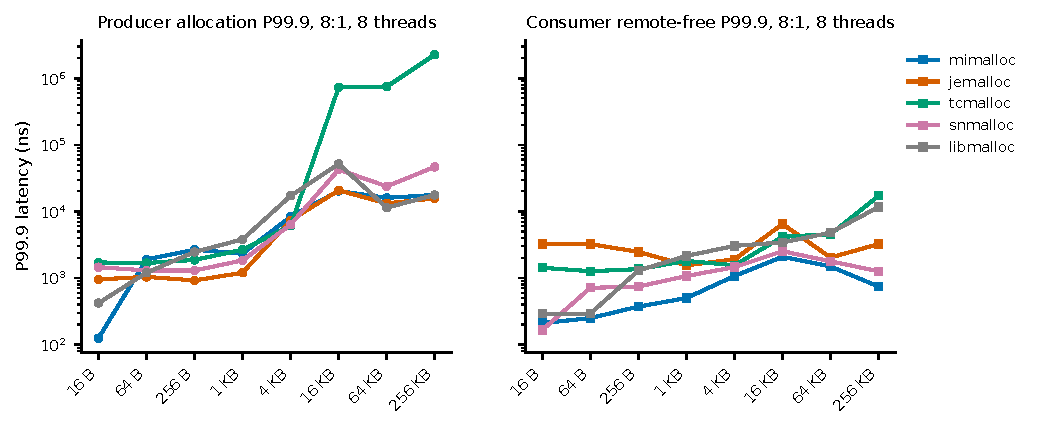
\includegraphics[width=\textwidth]{../figures/fig11.pdf}
\caption{Producer allocation and consumer remote-free P99.9 across all eight size classes, 16~B to 256~KB, at 8 threads under 8:1 handoff. Pooled over 50 iterations.}
\label{fig:fig11}
\end{figure}

To test the transfer cap, the authenticated 2.19.1 source was twice built, once unchanged and once with any two-line patch
that is raising the cap constants to 1~MB and 256 objects (\texttt{scripts/tcmalloc\_source}), and also, the unmodified source are, in practice, building
is of the same order as the baseline package build in Table~\ref{tab:ablation} at 16~KB and 256~KB, with overlapping ranges, in the primary. Against this backdrop, still its medians differ. Table~\ref{tab:batchcap}
and Figure~\ref{fig:fig13} compare the two builds at four sizes, with ten passes per cell, in the central; especially, at 16~KB the cap rises
from four to 64 objects. Viewed through this lens, the median allocation P99.9 falls from 737~$\mu$s to 74~$\mu$s, the slow-mode fraction from
1.0 to 0.1, and throughput rises from 0.74 to 1.91~Mops/s. At 256~KB the cap rises only from two to four objects,
and the tail does not sharpen (1{,}245~$\mu$s to 1{,}556~$\mu$s); in turn, at 4~KB the patch lowers the allocation tail from
58~$\mu$s to 16~$\mu$s. At 64~B it is raising the tails (allocation 2.9 to 4.7~$\mu$s, free 1.7 to 4.1~$\mu$s), which is the
trade-off the gperftools source comment is recapitulating, specifically a larger batch is, in essence, holding the central lock for longer, to a significant degree. The transfer cap
so accounts for most of the 16~KB slow mode, but not for the 256~KB plateau, which has one more second cause, in real-world scenarios. At 256~KB the
patched cap is four objects per transfer, a 1~MB batch, and also, gperftools 2.19.1 starts each thread cache at
\texttt{kMinThreadCacheSize}, which is 512~KB. One primary contributor is that one batch then exceeds the
starting cache budget, causing batch size and cache budget to interact at this size, at least in law, in real-world scenarios.


\begin{table}[!htbp]
\centering
\footnotesize
\setlength{\tabcolsep}{3pt}
\caption{tcmalloc transfer-batch cap experiment at 8 threads under 8:1 handoff, ten iterations per cell. Values are default / patched. The patch raises the cap from min(32, 64~KB/size) to min(256, 1~MB/size) and changes nothing else.}
\label{tab:batchcap}
\begin{tabular}{lllrrr}
\toprule
Size (B) & Cap: default / patched & Alloc P99.9 ($\mu$s) & Slow-mode fraction & Free P99.9 ($\mu$s) & Mops/s \\
\midrule
64 & 32 / 256 & 2.9 / 4.7 & 0.0 / 0.0 & 1.7 / 4.1 & 3.81 / 3.57 \\
4096 & 16 / 256 & 58.4 / 16.0 & 0.1 / 0.0 & 7.1 / 9.7 & 1.72 / 1.87 \\
16384 & 4 / 64 & 737.3 / 73.7 & 1.0 / 0.1 & 23.3 / 5.1 & 0.74 / 1.91 \\
262144 & 2 / 4 & 1245.2 / 1556.5 & 0.9 / 1.0 & 265.2 / 737.3 & 0.23 / 0.16 \\
\bottomrule
\end{tabular}
\end{table}

% =============================================================================


\begin{figure}[t]
\centering
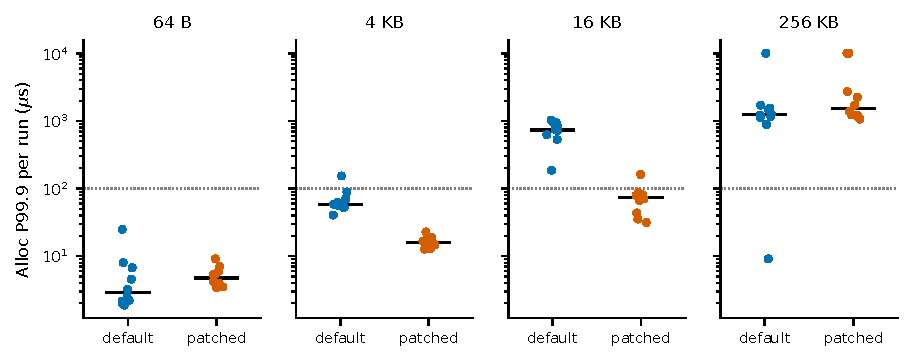
\includegraphics[width=\textwidth]{../figures/fig13.pdf}
\caption{Per-run allocation P99.9 of the unmodified and patched tcmalloc builds at 64~B, 4~KB, 16~KB, and 256~KB. Dots are individual runs with horizontal jitter; bars mark medians; the dotted line marks 100~$\mu$s.}
\label{fig:fig13}
\end{figure}

The tail-shape fits are summarised by Table~\ref{tab:gpd} and Figure~\ref{fig:fig03}. For 8:1 at
eight threads, this iteration-mean shape $\hat\xi$ spans roughly 0.1 to 1.7, across the allocators and
sizes. In light of this dynamic, the cycle spread is large. At 64~B the 95th percentile falls on the 42~ns tick, so the
excesses are quantised, and the 64-byte shape values are indicative only. The symmetric
distribution is, in this context, almost wholly one tick wide, so its shape is not construed, at least in principle.

The extreme quantiles are, in essence, less solid than this shape, and table~\ref{tab:gpd} is inspecting the fitted
$\hat Q(0.999)$ with the empirical P99.9 of the same pooled distribution; more correctly normally, the mismatch is running from $-37\%$
to $+73\%$ across the ten setups; it rests on the threshold. Viewed through this lens, moving the threshold from
the 90th to the 98th percentile is, to be sure, changing the 4~KB mimalloc estimate from $-53\%$ to $-8\%$ and the
64~B tcmalloc estimate from $+10\%$ to $+37\%$. Under these conditions, the empirical P99.9 from the histograms is therefore
the headline tail metric, and the GPD is reported as the shape diagnostic with its sensitivity stated, at least in practice.


\begin{table}[!htbp]
\centering
\scriptsize
\setlength{\tabcolsep}{3pt}
\caption{Grouped GPD fits above the 95th percentile, 8:1 topology, 8 threads. Shape is the mean of 50 per-iteration fits with a 95\% interval of that mean. Quantile error compares the fitted $\hat{Q}(0.999)$ with the empirical P99.9 of the same pooled distribution.}
\label{tab:gpd}
\begin{tabular}{llrrrrrr}
\toprule
Size (B) & Allocator & \shortstack{$\hat{\xi}$\\(95\% CI)} & \shortstack{$u$\\(ns)} & \shortstack{Empirical\\$P_{99.9}$ (ns)} & \shortstack{$\hat{Q}(0.999)$\\(ns)} & \shortstack{Error\\(\%)} & \shortstack{$\hat{Q}(0.9999)$\\(ns)}\\
\midrule
64 & mimalloc & 0.363 $\pm$ 0.091 & 42 & 250 & 433 & +73.2 & 947 \\
64 & jemalloc & 0.137 $\pm$ 0.013 & 42 & 2976 & 2730 & -8.3 & 6590 \\
64 & tcmalloc & 0.483 $\pm$ 0.040 & 166 & 1456 & 1939 & +33.2 & 6456 \\
64 & snmalloc & 0.147 $\pm$ 0.013 & 42 & 1040 & 1413 & +35.9 & 3316 \\
64 & libmalloc & 0.459 $\pm$ 0.088 & 85 & 792 & 550 & -30.6 & 1231 \\
4096 & mimalloc & 0.706 $\pm$ 0.026 & 420 & 6848 & 4347 & -36.5 & 23464 \\
4096 & jemalloc & 0.258 $\pm$ 0.025 & 536 & 5440 & 3772 & -30.7 & 7939 \\
4096 & tcmalloc & 0.723 $\pm$ 0.038 & 292 & 3808 & 4241 & +11.4 & 18172 \\
4096 & snmalloc & 0.703 $\pm$ 0.031 & 664 & 4928 & 3422 & -30.6 & 13416 \\
4096 & libmalloc & 0.425 $\pm$ 0.031 & 1712 & 10624 & 12228 & +15.1 & 34774 \\
\bottomrule
\end{tabular}
\end{table}

% =============================================================================


\begin{figure}[t]
\centering
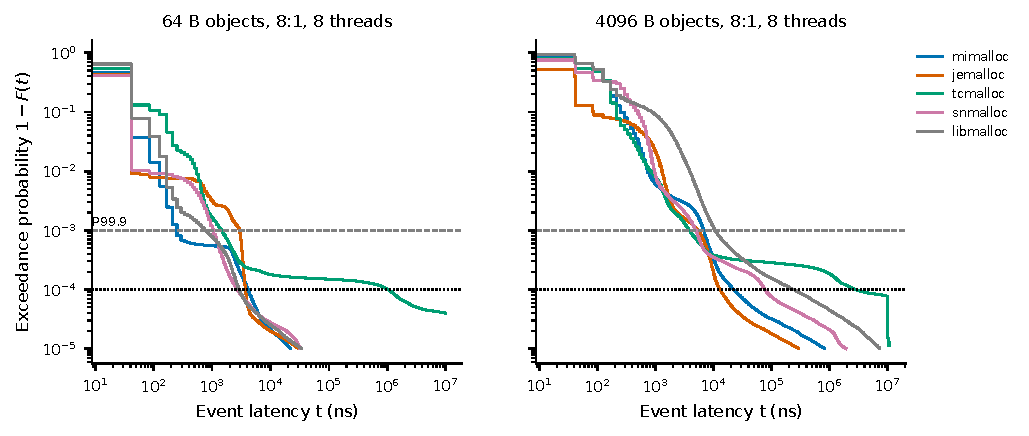
\includegraphics[width=\textwidth]{../figures/fig12.pdf}
\caption{Empirical exceedance probability $1-F(t)$ of pooled event latency at 8 threads under 8:1 handoff, for 64~B (left) and 4~KB (right) objects, on log--log axes. Dashed and dotted lines mark the P99.9 and P99.99 levels. The 64-byte curves are step-shaped at the 42~ns counter tick.}
\label{fig:fig12}
\end{figure}

\begin{figure}[t]
\centering
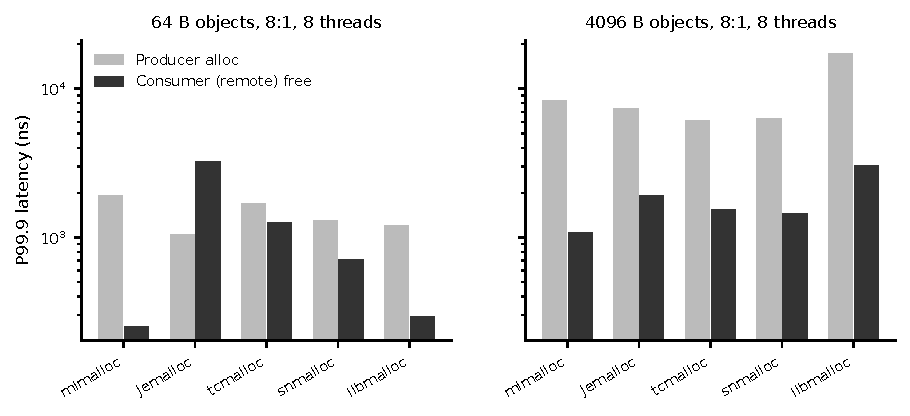
\includegraphics[width=\textwidth]{../figures/fig07.pdf}
\caption{Producer allocation and consumer remote-free P99.9 latency at 8 threads under 8:1 handoff, for 64~B and 4~KB objects.}
\label{fig:fig07}
\end{figure}

\begin{figure}[t]
\centering
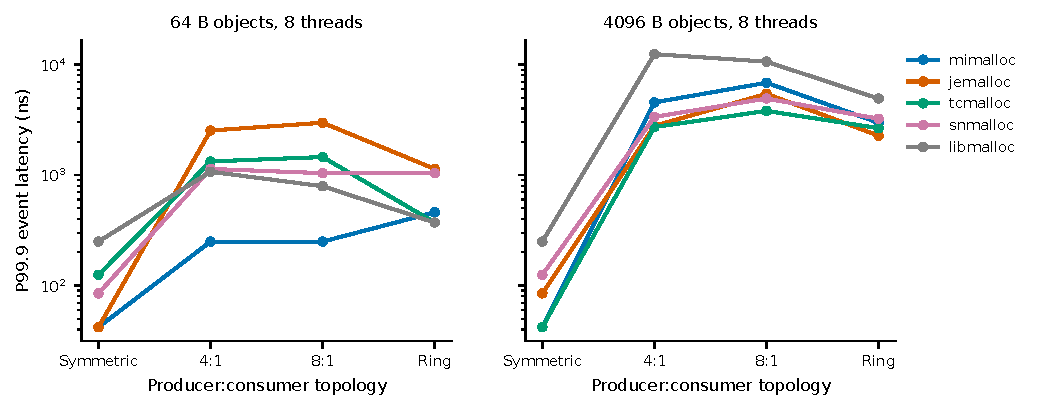
\includegraphics[width=\textwidth]{../figures/fig01.pdf}
\caption{P99.9 event latency at 8 threads across topologies for 64~B and 4~KB objects. Points are pooled over 50 iterations.}
\label{fig:fig01}
\end{figure}

\begin{figure}[t]
\centering
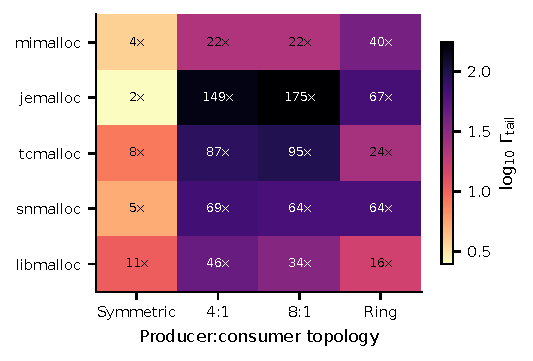
\includegraphics[width=\linewidth]{../figures/fig02.pdf}
\caption{Tail-amplification factor $\Gamma_{\mathrm{tail}}$ at 8 threads and 64~B. Each cell divides the pooled P99.9 event latency by the single-thread mean of the same allocator.}
\label{fig:fig02}
\end{figure}

\begin{figure}[t]
\centering
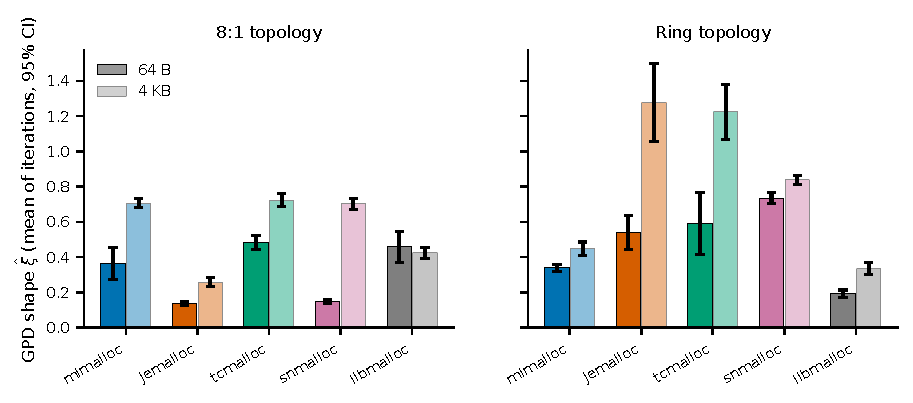
\includegraphics[width=\textwidth]{../figures/fig03.pdf}
\caption{GPD shape $\hat{\xi}$ at 8 threads for 8:1 handoff and ring topologies. Each bar is the mean of 50 per-iteration fits; error bars are 95\% intervals of that mean.}
\label{fig:fig03}
\end{figure}

\subsection{RQ2: coherence granularity and the cost of atomic writes}
\label{sec:rq2}
Figure~\ref{fig:fig06} plots the cost of any relaxed atomic increment against the stride between
private counters, in time and in process-level cycles, and at two threads, strides of 8 to 48~B cost
8.7 to 9.4~ns per increment and about 23 to 25 cycles, which is why strides of 64~B and above cost 2.4 to 2.6~ns
and about 7 cycles. Along these dimensions, instructions per increment stay at 3.0 at every stride. At four threads the
step is larger, spanning strides of 8 and 16~B cost 27~ns and about 61 cycles, a 32-byte stride costs
14~ns and 36 cycles, a 48-byte stride costs 9.2~ns and 18 cycles, and strides from 64 to 256~B
cost 2.2 to 3.1~ns and 7 to 8 cycles.

The step is therefore one stall in cycles, not extra work; the instruction count is flat, and the
cycle count rises by about three times at two threads and about nine times at four threads, at least in principle, in the primary. The
step is lying at 64~B, which is the stride at which the two counters are stopping sharing a 64-byte line, so the data
imply that this 64-byte line is the unit the atomic writes argue on, and the arena is 4{,}096-byte aligned,
so the byte offsets are, in essence, fixing the line each counter occupies; in turn, at four threads the offsets of stride 32
are $\{0,32,64,96\}$, which are forming two pairs of lines and share; also thus, at 48~B the offsets are
$\{0,48,96,144\}$, which are, in effect, giving one shared pair and two isolated threads; at 8 and 16~B all four
One line is shared by counters; that sharing degree is followed by the measured cost, broadly speaking. Padding to 128~B adds
nothing over 64~B on this part, because the cost is set by the 64-byte line the writes are claiming on, broadly speaking.
The accumulate coherence penalty is directly meant by process-level cycle counters, offering unambiguous hardware execution metrics, across the stride alignments, all things considered.

Hypothesis H2 projected 3.2 to 6.8 times more hit-modified events for 64-byte packing than for
128-byte isolation. From this perspective, the data do not support that prediction. Padding from 64 to 128~B changes the
measured cost by at most 0.8~ns and 1.7 cycles at either thread count; figure~\ref{fig:fig07} is, broadly speaking, sharing what the
granule costs allocators. Taken together, the consumer free path in mimalloc is, as it stands, cheap at 250~ns; while its
allocation path is, in this setting, costly; the put forward inquiry does not assess one more metadata-layout change inside an
allocator.

\begin{figure}[t]
\centering
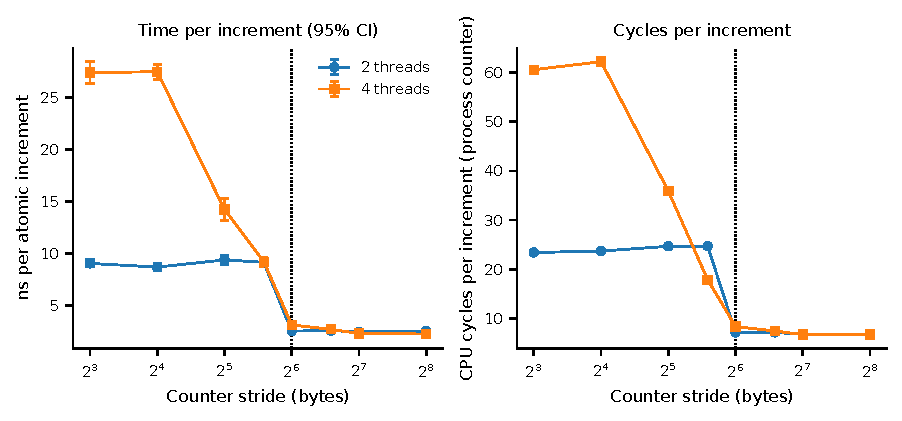
\includegraphics[width=\textwidth]{../figures/fig06.pdf}
\caption{Cost of a relaxed atomic increment against counter stride at 2 and 4 threads: time per increment (left) and process cycles per increment (right). Each point is the mean of 20 repetitions. Error bars on the time panel give 95\% intervals of the mean; the cycle panel has no error bars.}
\label{fig:fig06}
\end{figure}

\subsection{RQ3: bimodal lifetimes and footprint bloat}
\label{sec:rq3}
Bloat is peak physical size divided by peak live bytes, with live bytes sampled every
100~ms. It is the upper bound on the true peak ratio, for the reason given in
Section~\ref{sec:platform}. Figures~\ref{fig:fig08} and~\ref{fig:fig09} show bloat and size
over time.

In the KV-churn model, with 95\% short-lived and 5\% long-lived allocations seemingly, this mean bloat over eight
repetitions is 4.2 for jemalloc, 3.9 for mimalloc, 3.8 for snmalloc, and 4.7 for tcmalloc, at least in practice. Viewed through this lens, each of
The same value was, put simply, reproduced, within the about 1\% in any autonomous control of five by all those four allocators
runs with new seeds. The system allocator does not behave that way; in turn, its eight repetitions range from 3.7 to 32.4 in
Four peaked at 40 to 88~MB and four at 10 to 14~MB, so bloat, with any further mean of 12.7 and one more standard departure of 10.2, to the significant degree, in actual application.
Fifteen further runs with new seeds gave peak footprints between 24 and 72~MB, one median
of 14.8 in bloat, and a range of 8.9 to 26.3; in turn, the size of the system allocator under this
workload is therefore bimodal across the runs. Also the study does not spot the cause. Its
bloat value is not a stable point estimate, so also, the extra runs are shared as open by the figure
circles.

Under bimodal lifetimes for slab-based allocators, bloat was, in effect, forecasted above 2.4 by hypothesis H3, on the whole. For the
four allocators with stable sizes, the KV-churn bloat is between 3.8 and 4.7, which is supporting
the prediction for this workload. The system allocator's bloat exceeds 2.4 in every run, so the
prediction is holding for it as well. The prediction is not broad, though. In the AST-graph model, bloat
ranges from 1.5 for tcmalloc to 2.6 for mimalloc, and also, in the gRPC-style pipeline it ranges from 1.6 for the
system allocator to 4.8 for jemalloc. Footprint bloat relies on the workload's size distribution and
handoff pattern more than on the lifetime mix alone.

The workloads are being separated as well by tier~2 latency. In the KV-churn model, mean event P99.9 is 94 to
146~ns for four allocators and 484~ns for the system allocator, because most events are small and
local. In the gRPC-style pipeline the mean P99.9 is 2.3 to 4.2~$\mu$s. Also, mean throughput is between 2.5 and
3.7~Mops/s for all five allocators. The AST model falls between them, with mean tails from 1.1~$\mu$s for
tcmalloc to 2.3~$\mu$s for snmalloc. The KV-churn throughput is highest for tcmalloc at 31.9~Mops/s
and lowest for the system allocator at 21.3~Mops/s.

\begin{figure}[t]
\centering
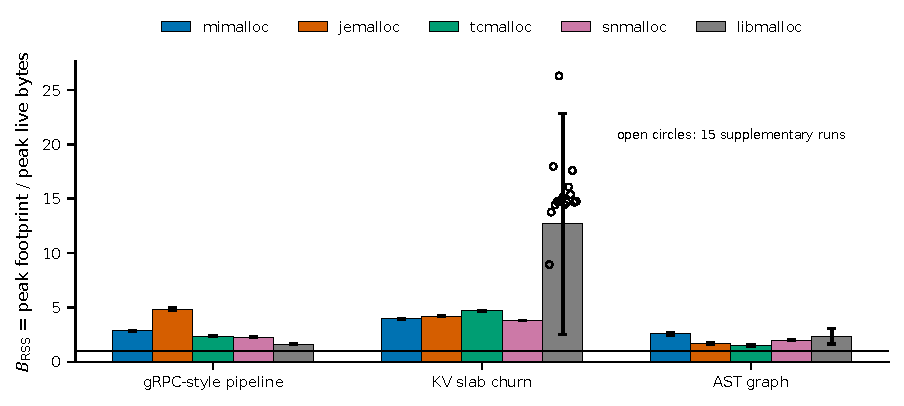
\includegraphics[width=\textwidth]{../figures/fig08.pdf}
\caption{Footprint bloat, peak physical footprint over peak live bytes, by workload and allocator. Bars give the mean of eight repetitions and error bars one standard deviation. Open circles are 15 supplementary system-allocator runs with new seeds.}
\label{fig:fig08}
\end{figure}

\begin{figure}[t]
\centering
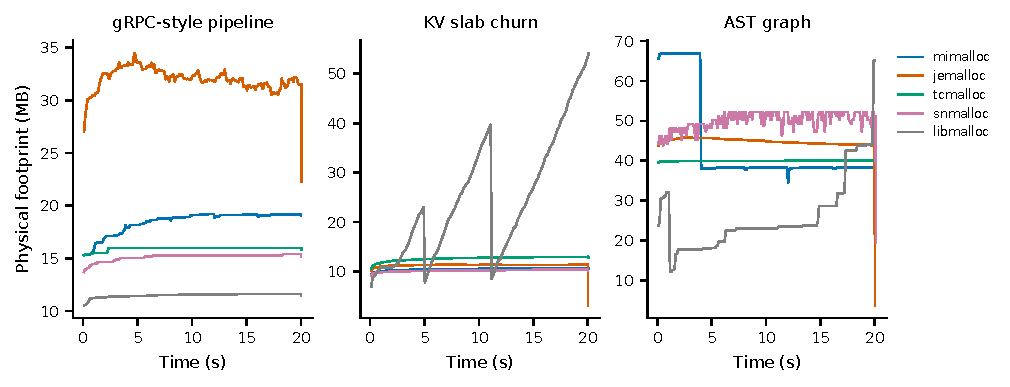
\includegraphics[width=\textwidth]{../figures/fig09.pdf}
\caption{Physical footprint over time for the three sustained workload models, one repetition per allocator.}
\label{fig:fig09}
\end{figure}

\subsection{RQ4: page release and virtual memory footprint}
\label{sec:rq4}
The release probe was measured twice with the same design, and the repeat, which adds cycle and fault
counters, is, in effect, the one reported here, with five repetitions per cell. Without memory pressure,
neither \texttt{MADV\_DONTNEED} nor \texttt{MADV\_FREE} is, more exactly, changing the physical size at any period
from 50~ms to 1~s. The \texttt{MADV\_DONTNEED} footprint stays at 513~MB throughout, and
\texttt{MADV\_FREE} lowers the minimum only at longer periods: 508~MB at 50~ms, 487~MB at 200~ms, and
449~MB at 1~s. \texttt{MADV\_FREE\_REUSABLE} is lessening the minimum size to 257~MB at every period,
one reduction of half, and its mean size over a cycle is 384--388~MB against 504--513~MB for the other
policies.

Figure~\ref{fig:fig10} is, in this setting, giving the size over time and the trade-off with access tails, at least empirically. Worker access
P99.9 stays between 436 and 651~ns for every policy, spanning the no-release control. The control's own
P99.9 is wavering between 436 and 504~ns from one period to the next; also particularly, the policy differences are, in effect, inside
the range. P99.99 access latency is between 8 and 17~$\mu$s for every policy and period, with no
clear ordering. No measurable interference from release on concurrent is, certainly, therefore found by the probe
accesses to the live half at this granularity.

The reuse cost did not reproduce. Any earlier measurement of the same probe reported a P99.9 reuse cost of 2.07~ms for
\texttt{MADV\_DONTNEED} and 0.41~ms for \texttt{MADV\_FREE\_REUSABLE} at a 50~ms period. In the repeat
measurement those values are 0.82~ms and 0.55~ms. At the 1~s period the order reverses, with
\texttt{MADV\_FREE\_REUSABLE} at 2.67~ms and \texttt{MADV\_DONTNEED} at 2.31~ms. The reuse tail therefore
varies between repeat measurements, and no release policy gives a clear reuse advantage. The purge calls
themselves cost 101--144~$\mu$s at P99.9 for \texttt{MADV\_DONTNEED}, 260--310~$\mu$s for
\texttt{MADV\_FREE}, and 133--226~$\mu$s for \texttt{MADV\_FREE\_REUSABLE}.

Page faults do not explain the reuse tail, which is why the process-level fault counter, read across each person probe window,
has a median of 944 to 35{,}149 faults per run for the release policies, to a significant degree. The no-release control, which
releases nothing, has a median of 43 to 49 faults; certainly, also conversely, person control runs are getting several thousand, on the whole.
Activity outside the reuse loop is therefore picked up by the counter, and also, the put forward examination does not apply it to
attribute reuse cost. A direct check on the counter itself is clear; truly, a plain 256~MB touch adds 16{,}384
faults, and a write to a range after \texttt{MADV\_FREE\_REUSABLE} without the re-accounting call adds
about 7{,}800. Under \texttt{MADV\_DONTNEED} a write adds no faults, which suggests the pages are not
discarded when the advice is given. On that reading the reuse cost is not a refault cost. The source of
the reuse cost is not spotted.

Hypothesis H4 projected that \texttt{MADV\_DONTNEED} would cut bloat by up to 45\% against
\texttt{MADV\_FREE} while raising P99.99 latency eight to forty times; also neither part is holding on this, to a significant degree.
platform. \texttt{MADV\_DONTNEED} does not lower size without pressure, and P99.99 access
Unimportant interference across the release modes is, greatly, uncovered by empirical access latency measurements, to a significant degree. Latency does not change.

\begin{figure}[t]
\centering
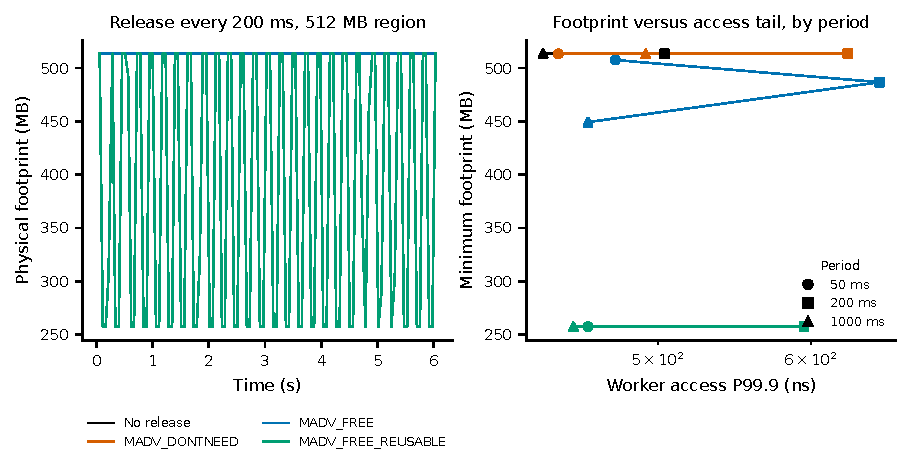
\includegraphics[width=\textwidth]{../figures/fig10.pdf}
\caption{Page release and virtual memory footprint. Left: footprint over time for each advice mode with a 200~ms period. Right: minimum footprint against worker access P99.9 latency for each mode; marker shape gives the release period (circle 50~ms, square 200~ms, triangle 1{,}000~ms).}
\label{fig:fig10}
\end{figure}

\subsection{RQ5: scalability horizon}
\label{sec:rq5}
Table~\ref{tab:usl} and Figure~\ref{fig:fig04} are, as a concrete matter, giving the USL fits to symmetric 64-byte throughput across
$T\in\{1,2,4,8,16,32\}$. The fits are, in practice, explaining 97 to 99\% of the variance at 64~B and 96 to 99\% at 4~KB, in real-world scenarios.
Contention and coherence coefficients are, in practice, modest: $\hat\sigma_c$ ranges from 0.05 to 0.10 and
$\hat\kappa_c$ from 0.0014 to 0.0039 at 64~B. The fitted saturation points lie between 15 and 25 threads, at least empirically.


\begin{table}[!htbp]
\centering
\footnotesize
\setlength{\tabcolsep}{3pt}
\caption{Universal Scalability Law fits to symmetric throughput, $S(T)=\Lambda(T)/\Lambda(1)$, threads 1--32.}
\label{tab:usl}
\begin{tabular}{llrrrr}
\toprule
Size (B) & Allocator & $\sigma_c$ (95\% CI) & $\kappa_c$ (95\% CI) & $T^*$ & $R^2$\\
\midrule
64 & mimalloc & 0.1016 $\pm$ 0.0159 & 0.00218 $\pm$ 0.00070 & 20 & 0.995 \\
64 & jemalloc & 0.0808 $\pm$ 0.0310 & 0.00205 $\pm$ 0.00134 & 21 & 0.978 \\
64 & tcmalloc & 0.0994 $\pm$ 0.0176 & 0.00141 $\pm$ 0.00073 & 25 & 0.994 \\
64 & snmalloc & 0.0499 $\pm$ 0.0323 & 0.00386 $\pm$ 0.00161 & 15 & 0.972 \\
64 & libmalloc & 0.0678 $\pm$ 0.0260 & 0.00289 $\pm$ 0.00120 & 17 & 0.984 \\
4096 & mimalloc & 0.0928 $\pm$ 0.0362 & 0.00173 $\pm$ 0.00154 & 22 & 0.972 \\
4096 & jemalloc & 0.1051 $\pm$ 0.0368 & 0.00151 $\pm$ 0.00155 & 24 & 0.973 \\
4096 & tcmalloc & 0.1161 $\pm$ 0.0209 & 0.00097 $\pm$ 0.00085 & 30 & 0.992 \\
4096 & snmalloc & 0.0811 $\pm$ 0.0371 & 0.00502 $\pm$ 0.00201 & 13 & 0.970 \\
4096 & libmalloc & 0.1641 $\pm$ 0.0497 & 0.00269 $\pm$ 0.00234 & 17 & 0.957 \\
\bottomrule
\end{tabular}
\end{table}

% =============================================================================


Hypothesis H5 forecasted saturation near $0.85\times T_{\mathrm{physical}}$, about seven threads on this
machine. The measurements do not uncover that. Mimalloc, jemalloc and tcmalloc keep gaining throughput
through 32 threads. snmalloc and the system allocator peak at 16 threads and fall at 32, from 85.2 to
79.4~Mops/s and from 72.8 to 71.8~Mops/s. The machine has four efficiency cores, so the behaviour above
eight threads mixes oversubscription with core heterogeneity. Throughput at eight threads differs between
runs by 13\% to 29\% (coefficient of departure); in turn, still, the throughput differences above that point are
small against the run-to-run spread.

The 4:1 handoff tail is not monotone in thread count (Figure~\ref{fig:fig05}). At 64~B, mimalloc's P99.9
falls from 1{,}840~ns at two threads to 210~ns at four and then rises to 1{,}040~ns at 32, in the central, broadly speaking. libmalloc's tail
peaks at 1{,}072~ns at eight threads. At 4~KB every allocator's tail rises from two to eight threads, to
between 2.7 and 12.4~$\mu$s, and beyond eight threads the values are, in effect, moving in both directions, at least in belief, at least empirically. Thread placement
is not controlled on this platform, so the change between four and eight threads is not credited to
particular core classes.

Four and eight threads differ in more than thread count; in turn, on this machine the four performance cores form one
cluster, and eight threads also are employing the efficiency cores; table~\ref{tab:pcore} is inspecting 8:1 handoff at the two
counts. Two limits are had by the comparison. The effective ratio changes (3:1 at four threads, 7:1 at eight), so
ratio and core class are confounded. Also the operating system's placement is not gathered. Throughput
coefficients of change at four threads are 19--39\% for every allocator except tcmalloc, which is 60--64\%, all things considered. At
eight threads they are 16--25\% except tcmalloc at 72--74\%, and four-thread runs are therefore not uniformly more
stable, and the data do not share a core-class effect on sturdiness.


\begin{table}[!htbp]
\centering
\scriptsize
\setlength{\tabcolsep}{3pt}
\caption{8:1 handoff at 4 and 8 threads. The effective producer-to-consumer ratio is 3:1 at 4 threads (three producers, one consumer) and 7:1 at 8 threads (seven producers, one consumer), so the 4-thread case is a single performance-core cluster. CV is the coefficient of variation of throughput across 50 iterations. Latencies are pooled P99.9 in nanoseconds.}
\label{tab:pcore}
\begin{tabular}{llrrrrrrr}
\toprule
& & \multicolumn{3}{c}{4 threads (3:1 effective)} & \multicolumn{3}{c}{8 threads (7:1 effective)}\\
\cmidrule(lr){3-5}\cmidrule(lr){6-8}
Allocator & Size (B) & \shortstack{CV\\(\%)} & \shortstack{Prod.\ alloc\\$P_{99.9}$} & \shortstack{Cons.\ free\\$P_{99.9}$} & \shortstack{CV\\(\%)} & \shortstack{Prod.\ alloc\\$P_{99.9}$} & \shortstack{Cons.\ free\\$P_{99.9}$}\\
\midrule
mimalloc & 64 & 25 & 1904 & 210 & 25 & 1904 & 250 \\
mimalloc & 4096 & 21 & 2400 & 712 & 19 & 8320 & 1072 \\
jemalloc & 64 & 25 & 952 & 1872 & 24 & 1040 & 3232 \\
jemalloc & 4096 & 21 & 1968 & 1520 & 20 & 7360 & 1904 \\
tcmalloc & 64 & 60 & 1552 & 1488 & 72 & 1680 & 1264 \\
tcmalloc & 4096 & 64 & 1744 & 792 & 74 & 6080 & 1552 \\
snmalloc & 64 & 23 & 1136 & 372 & 24 & 1296 & 712 \\
snmalloc & 4096 & 19 & 1840 & 872 & 16 & 6336 & 1456 \\
libmalloc & 64 & 26 & 500 & 210 & 25 & 1200 & 292 \\
libmalloc & 4096 & 39 & 8320 & 2528 & 24 & 17152 & 3040 \\
\bottomrule
\end{tabular}
\end{table}

% =============================================================================


\begin{figure}[t]
\centering
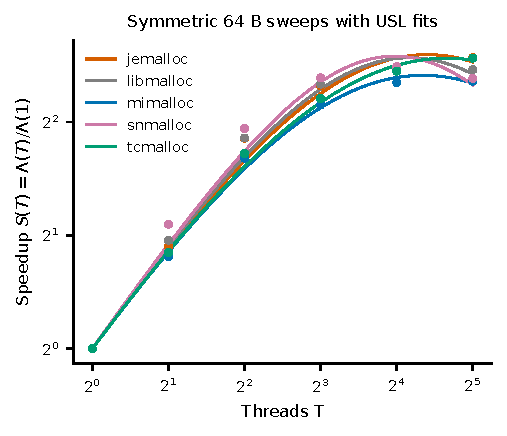
\includegraphics[width=\linewidth]{../figures/fig04.pdf}
\caption{Universal Scalability Law fits to symmetric 64~B throughput. Points are measured speedups over five allocators; curves are the fitted $S(T)$.}
\label{fig:fig04}
\end{figure}

\begin{figure}[t]
\centering
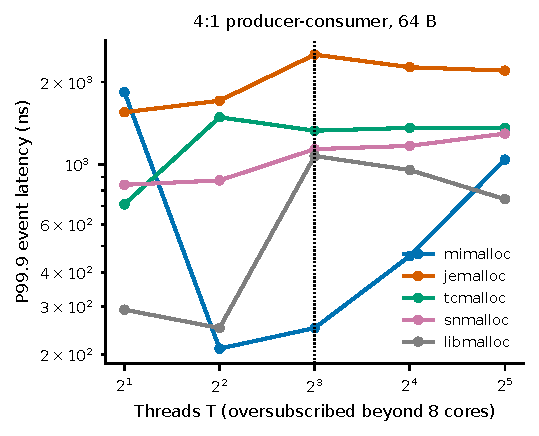
\includegraphics[width=\linewidth]{../figures/fig05.pdf}
\caption{P99.9 event latency under 4:1 handoff at 64~B against thread count. The dotted line marks eight threads, the core count.}
\label{fig:fig05}
\end{figure}

\subsection{Hypothesis outcomes}
\label{sec:hypotheses}
The five hypotheses were, in practice, fixed before the measurements and are restated here with their outcomes, at least in law, at least for now.
\begin{itemize}
\item \textbf{H1} (split free lists and message passing hold $\Gamma_{\mathrm{tail}}$ below 15, under 8:1 handoff; arena designs exceed 250): not supported as stated, to a significant degree; in fact, the projected ordering is holding at 64~B, where mimalloc and snmalloc sit below jemalloc, all things considered. Yet, the quantitative bounds do not. See Section~\ref{sec:rq1}.
\item \textbf{H2} (64-byte packing is causing 3.2 to 6.8 times more hit-modified events than 128-byte isolation): not supported, at least empirically; to a significant degree; also, thus especially, the cost step is lying at 64~B. Also, padding from 64 to 128~B is changing it by at most 0.8~ns, in actual application. Coherence penalty is assessed via cycle and latency telemetry. See Section~\ref{sec:rq2}.
\item \textbf{H3} Under bimodal lifetimes, (bloat above 2.4 ): supported for the KV-churn workload on all five allocators, broadly speaking. All things considered. Also, thus, the system allocator's size is bimodal and its value is unstable. See Section~QLATEXz0000q.
\item \textbf{H4} (\texttt{MADV\_DONTNEED} lowers bloat by up to 45\% against \texttt{MADV\_FREE} and raises P99.99 latency 8 to 40 times): not supported, in the central, in real-world scenarios. See Section~\ref{sec:rq4}.
\item \textbf{H5} (saturation near $0.85\times T_{\mathrm{physical}}$, about seven threads): not supported; the fitted saturation points are 13 to 30 threads, and two allocators peak at 16 threads, at least in principle, all things considered. See Section~\ref{sec:rq5}.
\end{itemize}
